\section{Experiments}\label{sec:experiments}
In this work, we take four applications including matrix multiplication (MM), FIR filter, Kmean and Sobel edge detector as our benchmark. To investigate the scalability of the accelerator design methods, each application is further provided with three different data sets ranging from small, medium to large ones. The basic parameters and configurations of the benchmark is illustrated in the \tabref{tab:benchmark-config}.

\begin{table*}[t]
  \caption{Detailed Configurations of the Benchmark}
  \label{tab:benchmark-config}
  \centering
  \begin{tabular}{c|c|c|c|c}
  \hline
  Benchmark & MM & FIR & Sobel & Kmean \\ \hline
  Parameters & Matrix Size & \tabincell{c}{\# of Input \\ \# of Taps+1} & \tabincell{c}{ \# of Vertical Pixels \\ \# of Horizontal Pixels} & \tabincell{c}{\# of Nodes \\ \# of Centroids \\ Dimension Size} \\ \hline
  Small & 10 & 40/50 & 8/8 & 20/4/2 \\ \hline
  Medium & 100 & 10000/50 & 128/128 & 5000/4/2  \\ \hline
  Large & 1000 & 100000/50 & 1024/1024 & 50000/4/2 \\ \hline
  \end{tabular}
\end{table*}

The benchmark is implemented on Zedboard using both Vivado HLS based design method and QuickDough. Then the design productivity, implementation efficiency and performance of the two design methods are compared respectively.

\subsection{Experiment Setup}
All the runtimes were obtained from a laptop with Intel(R) Core(TM) i5-3230M CPU and 8GB RAM. Vivado HLS 2013.3 is used to transform the compute kernel to hardware IP Catalog i.e. IP core. Vivado 2013.3 is used to integrate the IP core and build the FPGA accelertor. The SCGRA is initially developed in ISE 14.7, and then the ISE project is imported as an IP core in planAhead 14.7. With the SCGRA IP core, the SCGRA overlay based FPGA accelerator is further built in PlanAhead as well. Finally, the accelerators developed using both design methods target at Zedboard \cite{zedboard} and the system runs in the bare-metal mode.

Vivado HLS typically achieves the trade-off between hardware overhead and performance through altering the loop unrolling factors. Larger loop unrolling factors typically promise better performance, but this will not be guaranteed, because more hardware resources like DSP blocks will be required and the implementation frequency may degrade as well. In this work, we set the loop unrolling factor as large as possible and the detailed loop unrolling setup can be found in \tabref{tab:loop-unrolling-setup-vivado}.

As memory mapped IO buffers are used for the communication between FPGA and the accelerator, the compute kernel synthesized must have its input/output fully buffered. When the data set of the compute kernel is large, the on chip buffer will not be able to accommodate it. In this case, loop blocking is employed to divide the original compute kernel loop into loop blocks that fit the on-chip buffer. As presented in \tabref{tab:loop-unrolling-setup-vivado}, 2k-word buffer and 64k-word buffer will result in quite different blocking schemes for large data set. Since larger block size is beneficial to data reuse and amortizing the communication cost, the block size is set to be as large as possible within the on-chip buffer limit.

\begin{table*}[t]
\centering
\caption{Loop Unrolling \& Blocking Setup Of Accelerators Using Vivado HLS Based Design Method}
\label{tab:loop-unrolling-setup-vivado}
\begin{tabular}{|l|l|l|l|l|l|l|}
\hline
\multicolumn{2}{|l|}{\multirow{2}{*}{Application}} & \multicolumn{2}{l|}{Max-Buffer} & \multicolumn{2}{l|}{2k-Buffer} & \multirow{2}{*}{Complete Loop Structure} \\ \cline{3-6}
\multicolumn{2}{|l|}{} & Unrolling Factor & Block Structure & Unrolling Factor & Block Structure & \\ \hline
\multirow{3}{*}{MM} & Small & $2 \times 10 \times 10$ & $10 \times 10 \times 10$ & $2 \times 10 \times 10$ & $10 \times 10 \times 10$ & $10 \times 10 \times 10$ \\ \cline{2-7} 
                    & Medium & $1 \times 1 \times 100$ & $100 \times 100 \times 100$ & $1 \times 100$ & $10 \times 100$ & $100 \times 100 \times 100$ \\ \cline{2-7} 
                    & Large & $1 \times 500$ & $50 \times 1000$ & 500 & 1000  & $1000 \times 1000 \times 1000$ \\ \hline
\multirow{3}{*}{FIR} & Small & $2 \times 50$ & $40 \times 50$ & $2 \times 50$ & $40 \times 50$ & $40 \times 50$ \\ \cline{2-7} 
                     & Medium & $2 \times 50$ & $10000 \times 50$ & $2 \times 50$ & $1000 \times 50$ & $10000 \times 50$ \\ \cline{2-7} 
                     & Large & $2 \times 50$ & $50000 \times 50$ & $2 \times 50$ & $1000 \times 50$ & $100000 \times 50$ \\ \hline
\multirow{3}{*}{Sobel} & Small & $1 \times 2 \times 3 \times 3$ & $8 \times 8 \times 3 \times 3$ & $1 \times 2 \times 3 \times 3$ & $8 \times 8 \times 3 \times 3$ & $8 \times 8 \times 3 \times 3$ \\ \cline{2-7} 
                       & Medium & $1 \times 1 \times 3 \times 3$ & $128 \times 128 \times 3 \times 3$ & $1 \times 1 \times 3 \times 3$ & $23 \times 128 \times 3 \times 3$ & $128 \times 128 \times 3 \times 3$ \\ \cline{2-7} 
                       & Large & $1 \times 1 \times 3 \times 3$ & $75 \times 1024 \times 3 \times 3$ & $1 \times 1 \times 3 \times 3$ & $4 \times 1024 \times 3 \times 3$ & $1024 \times 1024 \times 3 \times 3$ \\ \hline
\multirow{3}{*}{KMean} & Small & $20 \times 4 \times 2$ & $20 \times 4 \times 2$ & $20 \times 4 \times 2$ & $20 \times 4 \times 2$ & $20 \times 4 \times 2$ \\ \cline{2-7} 
                       & Medium & $5 \times 4 \times 2$ & $5000 \times 4 \times 2$ & $5 \times 4 \times 2$ & $1000 \times 4 \times 2$ & $1000 \times 4 \times 2$ \\ \cline{2-7} 
                       & Large & $5 \times 4 \times 2$ & $25000 \times 4 \times 2$ & $5 \times 4 \times 2$ & $1000 \times 4 \times 2$ & $1000 \times 4 \times 2$ \\ \hline
\end{tabular}
\end{table*}

QuickDough has similar design choices to those of Vivado HLS based design method in terms of loop unrolling and blocking. However, the design constrains using the two design methods are different. The unrolled part in QuickDOugh is transformed to DFG which can further be scheduled to the SCGRA overlay, so the loop unrolling factor is mainly constrained by the resources of the SCGRA overlay such as SCGRA size, instruction memory size and data memory size. As for the loop blocking, the design constrain in QuickDough is relatively more complex. On the one hand, the block size is also limited by the size of input/output buffer, which is exactly the same with the constrain using Vivado HLS based design method. On the other hand, the address buffer size can be another major constrain, because we need to store all the IO buffer address sequence of the whole block instead of the DFG. Even though we set address buffer size twice larger than the data buffer size, it can still be a bottleneck in many occasions. The detailed SCGRA overlay configuration and corresponding loop unrolling as well as blocking setup using QuickDough are listed in \tabref{tab:scgra-config} and \tabref{tab:loop-unrolling-setup-scgra} respectively. 

\begin{table}[htb]
\caption{SCGRA Configuration}
\label{tab:scgra-config}
\centering
\begin{tabular}{|l|l|}

\hline
{SCGRA Topology} & {Torus} \\ \hline
{SCGRA Size} & {$2 \times 2$, $5 \times 5$} \\ \hline
{Data Wdith} & {32 bits} \\ \hline
{Instruction Length} & {72 bits} \\ \hline
{Instruction Memory Depth} & {1024} \\ \hline
{Data Memory Depth} & {256} \\ \hline
{Input/Output Buffer Depth} & {2048} \\ \hline
{Addr Buffer Depth} & {4096} \\ \hline

\end{tabular}
\end{table}

\begin{table*}[t]
\centering
\caption{Loop Unrolling and Blocking Setup For Accelerators Using QuickDough}
\label{tab:loop-unrolling-setup-scgra}
\begin{tabular}{|l|l|l|l|l|l|l|l|l|}
\hline
\multicolumn{2}{|l|}{\multirow{2}{*}{Application}} & \multicolumn{3}{l|}{SCGRA 2x2} & \multicolumn{3}{l|}{SCGRA 5x5} & \multirow{2}{*}{Complete Loop Structure} \\ \cline{3-8}
\multicolumn{2}{|l|}{} & Unrolling Factor & DFG(OP/IO) & Block Structure & Unrolling Factor & DFG(OP/IO) & Block Structure & \\ \hline
\multirow{3}{*}{MM} & Small & $10 \times 10 \times 10$ & 1000/301 & $10 \times 10 \times 10$ & $10 \times 10 \times 10$ & 1000/301 & $10 \times 10 \times 10$ & $10 \times 10 \times 10$ \\ \cline{2-9} 
            & Medium & $5 \times 100$ & 750/606 & $10 \times 100$ & $5 \times 100$ & 750/606 & $10 \times 100$ & $100 \times 100 \times 100$ \\ \cline{2-9} 
            & Large & 200 & 301/402 & 1000 & 200 & 301/402 & $10 \times 100$ & $1000 \times 1000 \times 1000$ \\ \hline
\multirow{3}{*}{FIR} & Small & $40 \times 50$ & 860/131 & $40 \times 50$ & $40 \times 50$ & 860/131 & $40 \times 50$ & $40 \times 50$ \\ \cline{2-9} 
                  & Medium & $20 \times 50$ & 1000/141 & $100 \times 50$ & $50 \times 50$ & 2500/201 & $250 \times 50$ & $10^4 \times 50$ \\ \cline{2-9} 
                  & Large & $20 \times 50$ & 1000/141 & $100 \times 50$ & $50 \times 50$ & 2500/201 & $250 \times 50$ & $10^5 \times 50$ \\ \hline
\multirow{3}{*}{Sobel} & Small & $4 \times 8 \times 3 \times 3$ & 1080/39 & $8 \times 8 \times 3 \times 3$ & $8 \times 8 \times 3 \times 3$ & 2160/55 & $8 \times 8 \times 3 \times 3$ & $8 \times 8 \times 3 \times 3$  \\ \cline{2-9} 
                  & Medium & $4 \times 8 \times 3 \times 3$ & 1080/39 & $8 \times 8 \times 3 \times 3$ & $23 \times 8 \times 3 \times 3$ & 6210/115 & $65 \times 8 \times 3 \times 3$ & $128 \times 128 \times 3 \times 3$ \\ \cline{2-9} 
                  & Large & $4 \times 4 \times 3 \times 3$ & 540/31 & $16 \times 4 \times 3 \times 3$ & $16 \times 4 \times 3 \times 3$ & 2160/55 & $16 \times 4 \times 3 \times 3$ & $1024 \times 1024 \times 3 \times 3$  \\ \hline
\multirow{3}{*}{KMean} & Small & $20 \times 4 \times 2$ & 920/62 & $20 \times 4 \times 2$ & $20 \times 4 \times 2$ & 920/62 & $20 \times 4 \times 2$ & $20 \times 4 \times 2$ \\ \cline{2-9} 
                 & Medium & $25 \times 4 \times 2$ & 1144/72 & $125 \times 4 \times 2$ & $125 \times 4 \times 2$ & 5768/272 & $500 \times 4 \times 2$ & $5000 \times 4 \times 2$ \\ \cline{2-9} 
                 & Large & $25 \times 4 \times 2$ & 1144/72 & $125 \times 4 \times 2$ & $125 \times 4 \times 2$ & 5768/272 & $500 \times 4 \times 2$ & $50000 \times 4 \times 2$  \\ \hline
\end{tabular}
\end{table*}

\subsection{Experiment Results}
In this section, design productivity, hardware implementation efficiency, performance and scalability of the accelerators using both design methodologies are presented and compared. 

\subsubsection{Design Productivity}
Design productivity involves many different aspects such as the abstraction level of the design entry, compilation time, design reuse, and design portability, and it is difficult to compare all the aspects, especially some of the aspects could hardly be quantized. In this section, we mainly concentrate on the compilation time comparison and analyze the rest briefly.

In order to develop an FPGA accelerator for an application, Vivado HLS based design method roughly consists of the following four steps including compute kernel synthesis, kernel IP generation, overall system implementation and software compilation. At the compute kernel synthesis step, high level language program kernel is translated to an HDL model according to the user's synthesis pragma. The next step is to further synthesize it and have it packed as an IP core. At the same time, the timing constrain should be met and the corresponding driver should be generated. Afterwards, the IP core can be integrated into the accelerator and the whole accelerator can be implemented on the FPGA accordingly. Finally, the application employing the FPGA accelertor should be compiled to binary code as conventional software.

The FPGA accelerator developed using QuickDough also needs four steps to complete the application acceleration. The first step is to translate the high level language program kernel to DFG. The second step is to schedule the DFG to the customized SCGRA overlay and dump the scheduling result for the following step. The third step is to integrate the scheduling result and the pre-built accelerator bitstream to produce the new bitstream for target application. Finally, the last step is also a conventional software compilation, which is similar to the fourth compilation step of the Vivado HLS based design method. 

\figref{fig:Vivado-HLS-Compilation-Time} and \figref{fig:SCGRA-Overlay-Compilation-Time} present the compilation time of implementing the benchmark using both Vivado HLS based design method and QuickDough respectively. IP core generation and hardware implementation in Vivado HLS based design method is relatively slow. Compute kernel synthesis is usually as fast as the software compilation and can be done in a few seconds, but it may take up to 10 minutes when there is pipelined large loop unrolling involved. The last step is essentially a software compilation, and the time consumed can be negligible. On the whole, the design method takes 20 minutes to an hour to implement an application. With pre-implemented SCGRA overlay, the processing steps except the DFG scheduling of QuickDough are fast and don't change much across the different applications. DFG scheduling is relatively slower especially when the DFG size and CGRA size are large, but it can still be completed in a few seconds. Basically, QuickDough could implement an application in 5 to 15 seconds and it is two magnitude faster than the SCGRA overlay based design method. 

\begin{figure}[htb]
\center{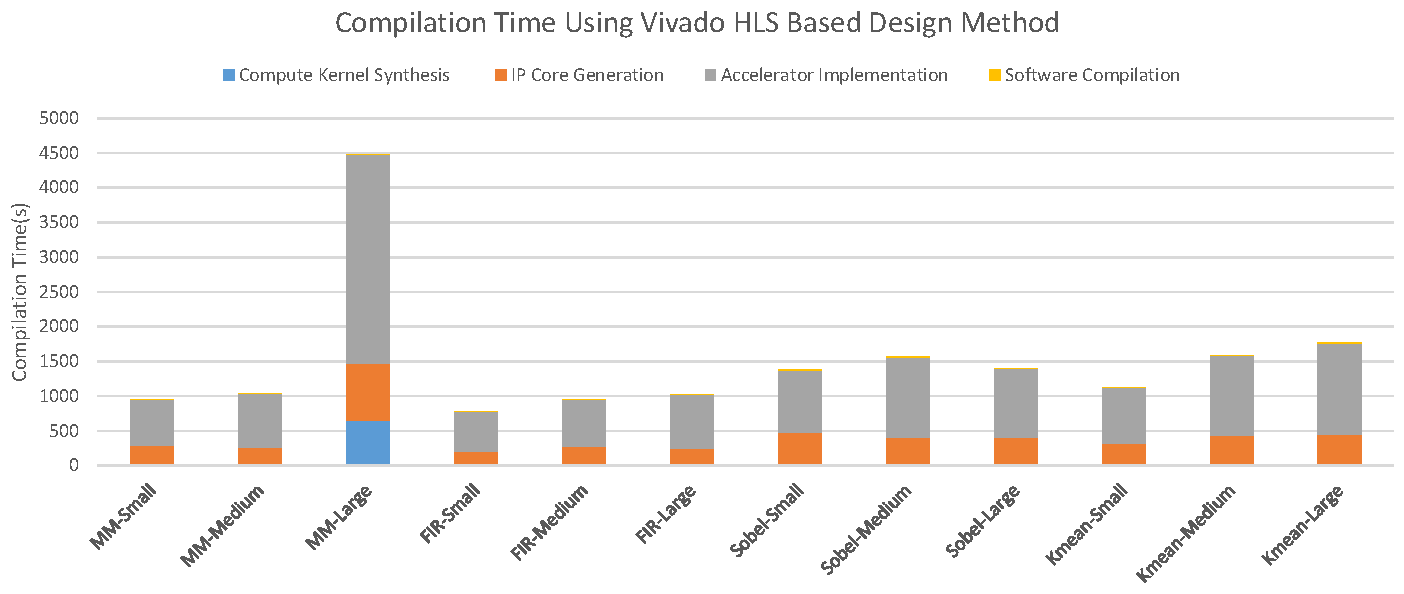
\includegraphics[width=1\linewidth]{HLS-Compilation-Time}}
\caption{Benchmark Compilation Time Using Vivado HLS Based Design Method}
\label{fig:Vivado-HLS-Compilation-Time}
\end{figure}

\begin{figure}[htb]
\center{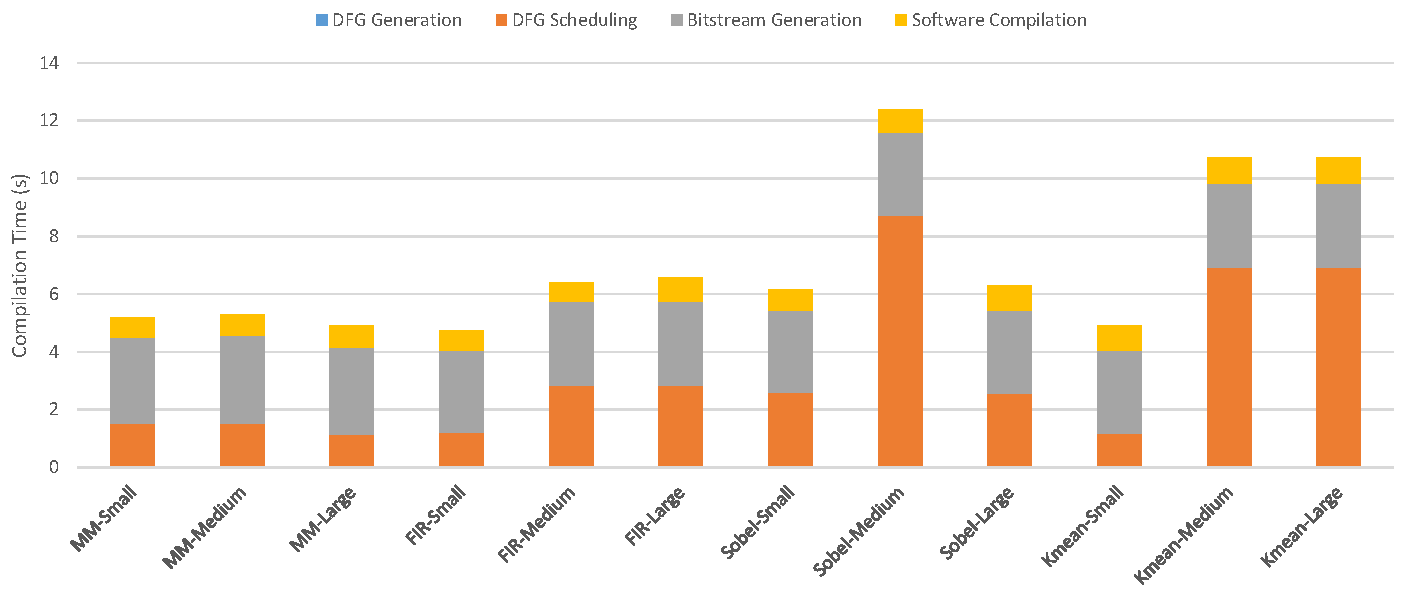
\includegraphics[width=1\linewidth]{QuickDough-Compilation-Time}}
\caption{Benchmark Compilation Time Using QuickDough}
\label{fig:SCGRA-Overlay-Compilation-Time}
\end{figure}

On top of the compilation time, the abstraction level of the design entry, design reuse and portability are also important aspects that influence the design productivity. Both Vivado HLS based design method and QuickDough adopt sequential high level language C/C++ as design input, but QuickDough still needs further efforts to have the DFG generation done automatically. Vivado HLS based design method needs the compute kernel be synthesized and implemented for each application instance. QuickDough requires compilation for each application instance as well, but could reuse the same hardware infrastructure across the applications in the same domain. It is possible for Vivado HLS based design method to port the synthesized HDL design among different devices and parts, but IP core generation and accelerator implementation depend on specific FPGA device. QuickDough's portability is also limited at HDL level, and complete hardware implementation is needed to port to a different FPGA device.

\subsubsection{Hardware Implementation Efficiency}
In this section, hardware implementation efficiency including the hardware resource overhead and implementation frequency of the accelerators using both Vivado HLS based design method and QuickDough are compared. 

\tabref{tab:hardware-overhead-comparison} exhibits the hardware overhead using both accelerator design methods. It is clear that the accelerators using Vivado HLS based design method typically consume less FF, LUT and RAM36 due to the delicate customization for each application configuration. However, the number of DSP48 required increases dramatically with the expansion of the application kernel and it limits the maximum loop unrolling factors for many applications. The accelerators using QuickDough usually cost comparable DSP48, more FF, LUT and particularly RAM36. Taking consideration of the total resource on FPGA, the overhead of DSP48, FF and LUT are still acceptable, while the RAM36 consumption is really large and it limits the maximum SCGRA that can be implemented on the target FPGA. Accordingly, it further constrains the maximum loop unrolling and blocking as well.

\begin{table}[htb]
\centering
\caption{Hardware Overhead of The Accelerators Using Both Vivado HLS Bsed Design Method and QuickDough}
\label{tab:hardware-overhead-comparison}
\begin{tabular}{l|l|l|l|l|l|l}
\hline
\multicolumn{3}{l|}{} & FF  & LUT & RAM36 & DSP48 \\ \hline 
\multirow{6}{*}{MM} & \multirow{3}{*}{ \tabincell{c}{2K \\ Buffer}} & Small & 4812 & 3390 & 4 & 84 \\ \cline{3-7} 
                    &                            & Medium & 4804 & 4703 & 4 & 12 \\ \cline{3-7} 
                    &                            & Large & 11107 & 11524 & 4 & 12 \\ \cline{2-7}
                    & \multirow{3}{*}{ \tabincell{c}{Max \\ Buffer}} & Small & 4826 & 3390 & 128 & 84 \\ \cline{3-7} 
                    &                             & Medium &  4251 & 4866 & 128 & 9 \\ \cline{3-7} 
                    &                             & Large & 11024 & 24890 & 128 & 12 \\ \hline

\multirow{6}{*}{FIR} & \multirow{3}{*}{ \tabincell{c}{2K \\ Buffer}} & Small & 3736 & 3570 & 4 & 27 \\ \cline{3-7} 
                     &                            & Medium & 3756 & 3872 & 4 & 27  \\ \cline{3-7} 
                     &                            & Large & 3756 & 3872 & 4 & 27 \\ \cline{2-7}
                     & \multirow{3}{*}{ \tabincell{c}{Max \\ Buffer}} & Small & 3742  & 3570 &  128 & 27 \\ \cline{3-7} 
                     &                             & Medium & 3782 & 4246 & 128 & 27 \\ \cline{3-7} 
                     &                             & Large & 3792 & 4426 & 128 & 27 \\ \hline

\multirow{6}{*}{Sobel} & \multirow{3}{*}{ \tabincell{c}{2K \\ Buffer}} & Small & 9556 & 6467 & 6 & 216 \\ \cline{3-7} 
                       &                            & Medium & 7483 & 5520 & 6 & 144 \\ \cline{3-7} 
                       &                            & Large & 7102 & 5501 & 6 & 144 \\ \cline{2-7}
                       & \multirow{3}{*}{ \tabincell{c}{Max \\ Buffer}} & Small & 9564 & 6467 & 130 & 216 \\ \cline{3-7} 
                       &                             & Medium & 7496 & 5711 & 130 & 144 \\ \cline{3-7} 
                       &                             & Large & 7622 & 5904 & 130 & 144 \\ \hline

\multirow{6}{*}{Kmean} & \multirow{3}{*}{ \tabincell{c}{2K \\ Buffer}} & Small & 2826 & 3567 & 4 & 24 \\ \cline{3-7} 
                       &                            & Medium & 6709 & 8088  & 4 & 120 \\ \cline{3-7} 
                       &                            & Large & 6709  & 8088  & 4  & 120 \\ \cline{2-7}
                       & \multirow{3}{*}{ \tabincell{c}{Max \\ Buffer}} & Small & 2852 & 3567 & 128 & 24 \\ \cline{3-7} 
                       &                             & Medium & 6754 & 8122 & 128 & 120 \\ \cline{3-7} 
                       &                             & Large & 6770 & 8205 & 128 & 120 \\ \hline

\multicolumn{2}{l|}{SCGRA 2x2} & 9302 & 5745 & 32 & 24  \\ \hline
\multicolumn{2}{l|}{SCGRA 5x5} & 34922 & 21436 & 137 & 150 \\ \hline
\multicolumn{2}{l|}{FPGA Resource} & 106400 & 53200 & 140 & 220 \\ \hline
\end{tabular}
\end{table}

\figref{fig:impl-freq} presents the implementation frequency of the benchmark using both accelerator design methods. Vivado HLS based design method takes timing constrain into consideration at the HLS step, and it could either synthesize the compute kernel to a lower frequency design with better simulation performance or a higher frequency design with worse simulation performance. Neither of them have a clear advantage over the other. While the AXI controller could work at around 100MHz by default and higher frequency design requires delicate placing and routing. Eventually, we set the HLS timing constrain at 100MHz and the whole accelerator could be synchronous. As there are so many different design options, the current design is not necessarily the optimal one, but it is representative. In addition, the synthesized IP core sometimes can be even slower though we set the timing at 100MHz during HLS. In this case, we don't spend time iterating the the HLS and implementing the whole design again. Instead, we just slow down the clock frequency until the timing constrain is met. As a result, sometimes the accelerator can only work at around 60MHz.

QuickDough utilizes the SCGRA overlay as the hardware infrastructure. Since the SCGRA overlay is regular and pipelined, the implementation frequency of the accelerator built on top of the SCGRA overlay is much higher than that of the accelerator produced using Vivado HLS. A 2x2 SCGRA based accelerator could run at 200MHz, and a 5x5 SCGRA based accelerator could work at 167MHz. The implementation frequency degrades slightly, because more than 95\% of the BRAM blocks on target FPGA are used and the routing becomes extremely tight. However, the AXI controller block on Zedboard is slower and runs around 100MHz. To take advantage of the higher implementation frequency, simple synchronizers built with consecutive registers are inserted to divide the AXI controller and the SCGRA overlay into two separate clock domains. Also note that the implementation frequency of the SCGRA based accelerators in \figref{fig:impl-freq} actually refers to the SCGRA overlay.

\begin{figure*}[h]
\center{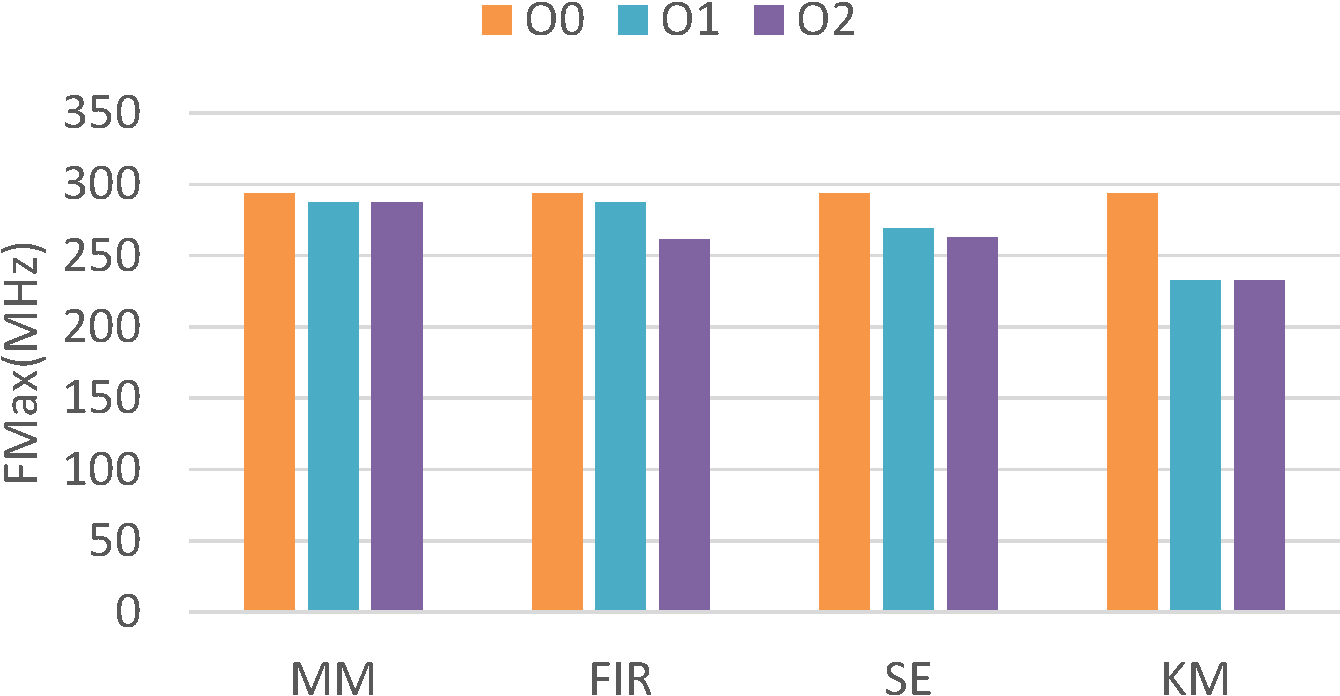
\includegraphics[width=0.75\linewidth]{impl-freq}}
\caption{Implementation Frequency of The Accelerators Using Both Vivado HLS Based Design Method and QuickDough}
\label{fig:impl-freq}
\end{figure*}

\subsubsection{Performance}
In this section, the execution time of the benchmark is taken as the performance metric. Since the execution time of different applications and data sets varies a lot, the performance speedup relative to Vivado HLS based implementation with 2k-Buffer configuration is used instead. \figref{fig:real-perf} shows the performance comparison of four different sets of accelerator implementations including two accelerators built with QuickDough and two accelerators developed with Vivado HLS based design method. According to this figure, Vivado HLS based design method wins the MM-Medium, MM-Large, Sobel-Medium and Sobel-Large, while QuickDough outperforms in FIR with all three data sets, Kmean-Medium and Kmean-Large. The two design methods achieve similar performance on the rest of the benchmark. 

\begin{figure*}[h]
\center{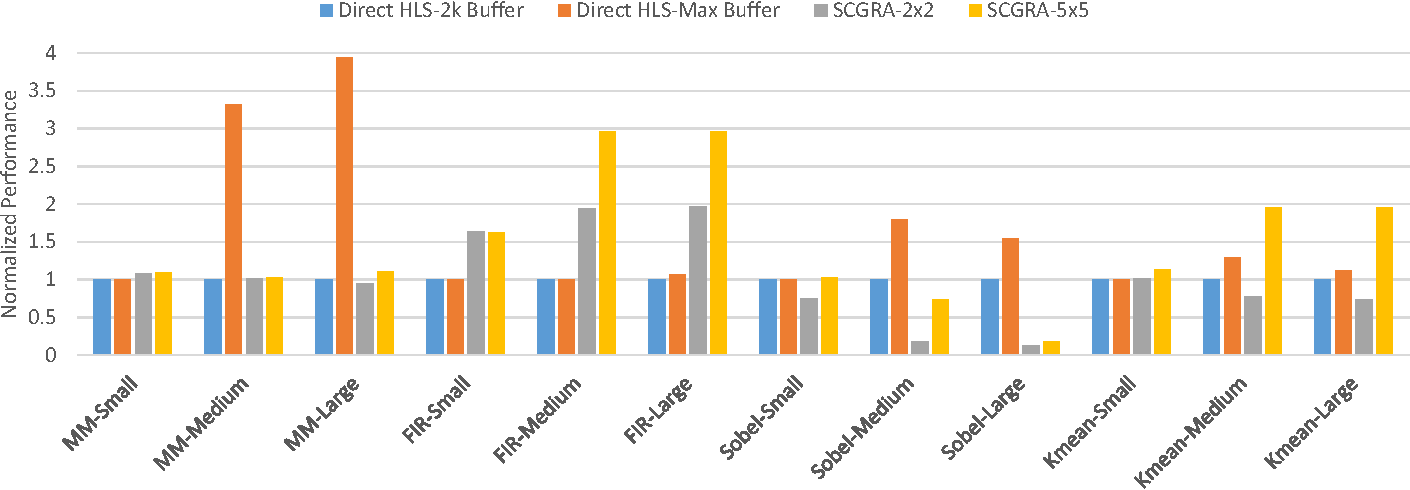
\includegraphics[width=0.75\linewidth]{real-perf}}
\caption{Benchmark Performance Using Both Vivado HLS Based Design Method and QuickDough}
\label{fig:real-perf}
\end{figure*}

To gain insight into the performance of the two design methods, \figref{fig:execution-time} presents the execution time decomposition of the benchmark. As the execution time of different applications with diverse data sets varies in a large range. To fit all the data in a single figure, the execution time used in this figure is actually normalized to that of a basic software implementation on ARM. The benchmark runs on an ARM + FPGA architecture where FPGA handles the compute kernel leaving the rest on ARM processor, the execution of the benchmark can be roughly divided into four parts: system initialization such as DMA initialization, communication between FPGA and ARM processor moving input/output data to/from the FPGA on-chip buffers, FPGA computation and the others such as input/output data reorganization for DMA transmission or corner case processing. 

According to this figure, accelerators using Vivado HLS based desgin method especially the one with max-buffer configuration perform better performance mainly due to the smaller overhead in communication and the others which are essentially the input/output data reorganization time. As presented in \tabref{tab:loop-unrolling-setup-vivado}, it is clear that accelerators using Vivado HLS based design method with max-buffer configuration could accommodate larger data sets and corresponding computation as well, which may improve the data reuse of the communication and deduce the amount of communication and data reorganization cost. This is one of the major reasons for lower communication cost while using Vivado HLS based design method. Moreover, part of the DMA transmission cost probably induced by DMA initialization routine is independent on the transmitted data size. Therefore, the average communication cost per data can be lower when the data size per DMA transmission is larger. Of course, the benefit will be negligible when the DMA transmission size is big enough to amortize the initialization cost. Because of the reasons mentioned above, for all the applications of the benchmark with medium and large data sets, the accelerators using Vivado HLS based design method especially with the Max-Buffer configuration have smaller communication and data reorganization cost.

\begin{figure*}[h]
\center{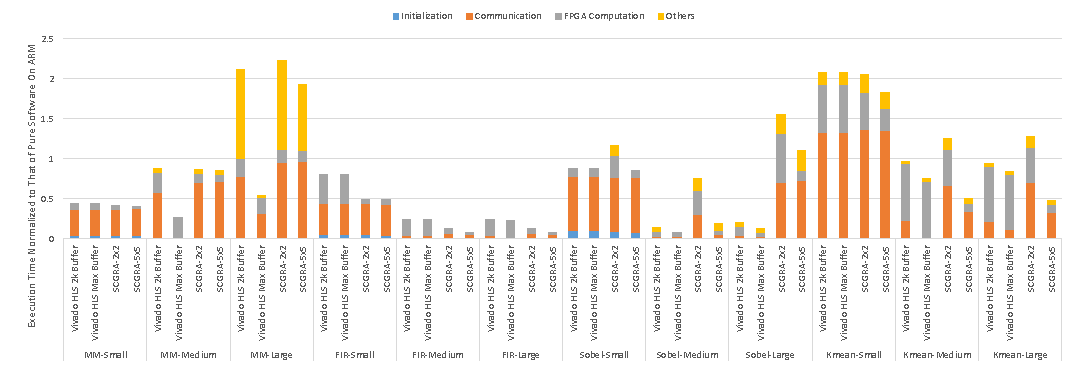
\includegraphics[width=0.95\linewidth]{execution-time}}
\caption{Benchmark Execution Time Decomposition Of The Accelerators Using Both Vivado HLS Based Design Method and QuickDough}
\label{fig:execution-time}
\end{figure*}

Computation time is crucial to the overall execution time. It basically depends on both the simulation performance in cycles and implementation frequency of the hardware infrastructure. \figref{fig:kernel-sim-perf} shows the simulation performance which is the product of the block simulation performance and the number of blocks for each application. From this paper, it is clear that Vivado HLS based design method wins on MM-Large and Sobel while QuickDough outperforms on the rest of the benchmark. Referring to both the simulation performance in this figure and loop unrolling factors in \tabref{tab:loop-unrolling-setup-vivado} and \tabref{tab:loop-unrolling-setup-scgra}, it can be found that the simulation performance is quite relevant to the depth of the loop unrolling. More precisely, the simulation performance mostly depends on the depth of the loop unrolling instead of the specific hardware infrastructure. The only exception is the Sobel benchmark. QuickDough performs more intensive loop unrolling, but the simulation performance is not as good as Vivado HLS. The reason is probably due to the two Sobel operators used in the algorithm. Vivado HLS takes them as constant input and could have special optimization on it. While the DFG generator in QuickDough just takes them as normal variable input and more operations are required. 

Loop unrolling factor is crucial to the simulation performance of the compute kernel, while the hardware infrastructure determines how much the loop can be unrolled, which eventually influences the simulation performance of the compute kernel. As presented in \tabref{tab:loop-unrolling-setup-vivado} and \tabref{tab:loop-unrolling-setup-scgra}, the loop unrolling factor with Vivado HLS is smaller than that in QuickDough in many cases. And this explains the comparison of the simulation performance using the two design methods.

QuickDough using SCGRA overlay as the hardware infrastructure could run at higher frequency, and the advantage of computation time as shown in \figref{fig:kernel-real-perf} is enlarged on top of that in the simulation performance. 

\begin{figure*}[h]
\center{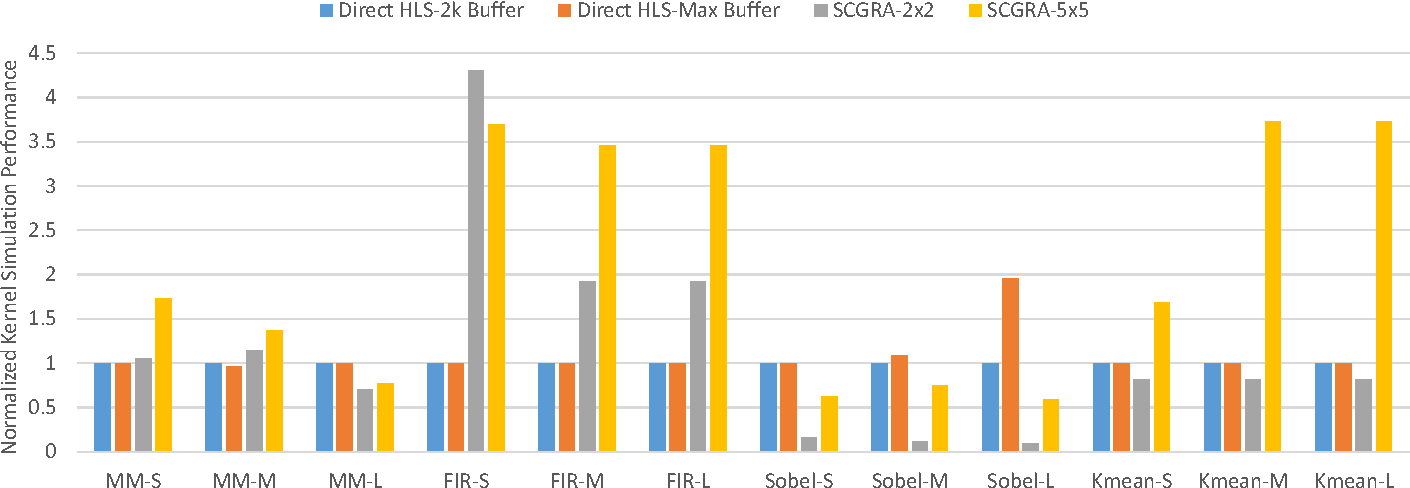
\includegraphics[width=0.75\linewidth]{kernel-sim-perf}}
\caption{Simulated Compute Kernel Performance Using Both Vivado HLS Based Design and QuickDough}
\label{fig:kernel-sim-perf}
\end{figure*}

In summary, the accelerators using Vivado HLS based design method could afford larger buffer and accommodate larger block size, which helps to reduce the communication time and the cost of input/output organization. Therefore, when there are more data reuse among neighboring blocks, the accelerators using Vivado HLS based design method achieves better performance. QuickDough using SCGRA overlay could provide both higher simulation performance with larger loop unrolling capability in many cases and higher implementation frequency due to its regular structure, so it wins when the target application has smaller data set or more intensive computation.  

\begin{figure*}[h]
\center{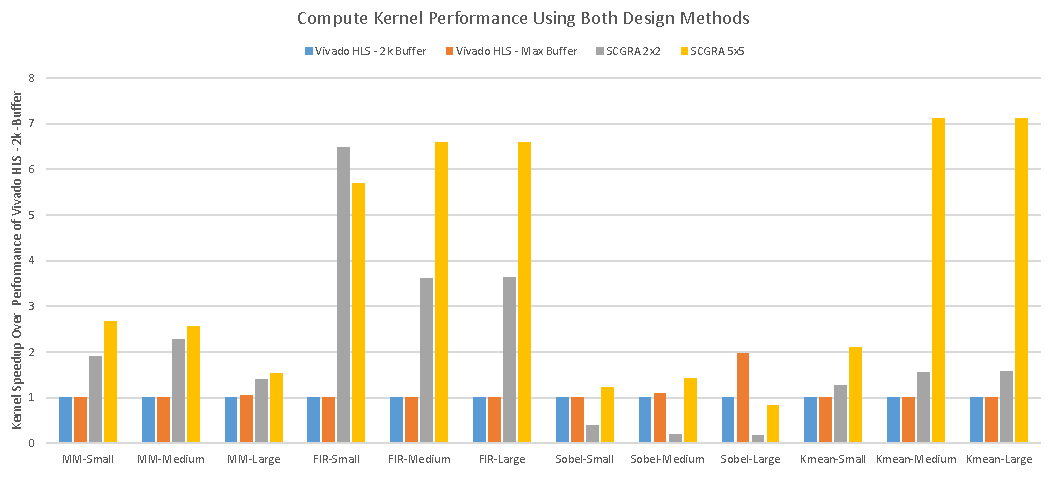
\includegraphics[width=0.75\linewidth]{kernel-real-perf}}
\caption{Compute Kernel Performance Using Both Vivado HLS Based Design Method and QuickDough}
\label{fig:kernel-real-perf}
\end{figure*}

\subsubsection{Scalability}
On top of the design productivity, hardware implementation, and performance, the scalability of the accelerator using the design methods is also equally important. To investigate the scalability of the accelerators using both design methods, we adopt matrix multiplication with smoothly increasing matrix size as the benchmark. 
